\documentclass[11pt]{article}
\usepackage[review]{acl}
\usepackage{times}
\usepackage{latexsym}
\usepackage[T1]{fontenc}
\usepackage[utf8]{inputenc}
\usepackage{microtype}
\usepackage{inconsolata}
\usepackage{booktabs}
\usepackage{multirow}
\usepackage{array}
\usepackage{tabularx}
\usepackage{graphicx}
\usepackage{amsmath}
\usepackage{amssymb}
\usepackage{xcolor}
\usepackage{url}
\usepackage{pgfplots}
\pgfplotsset{compat=1.18}
\usepackage{pgfplotstable}
\usepgfplotslibrary{groupplots,statistics}
\usepackage{adjustbox}
\setlength{\emergencystretch}{2em}

\newcommand{\method}{ConflictRAG}
\newcommand{\syntheticlabel}{Synthetic example result - replace before submission}
\newcommand{\todoexp}[1]{\textcolor{red}{[TODO: #1]}}
\newcolumntype{L}[1]{>{\raggedright\arraybackslash}p{#1}}

\title{ConflictRAG: Policy Evaluation for Retrieval-Augmented Generation with Conflicting Evidence}
\author{Anonymous EMNLP Submission \\ Paper ID: TBD}

\begin{document}
\maketitle

\begin{abstract}
Retrieval-augmented generation systems routinely produce confident, fluent responses even when the retrieved evidence is internally conflicting, topically irrelevant, or too sparse to ground a reliable answer---a miscalibration that directly causes hallucination in high-stakes deployments. Existing approaches address retrieval quality or post-hoc hallucination detection in isolation, but no prior work treats the response policy itself as the object of study. We introduce \method{}, a training-free, CPU-deployable framework that extracts four retrieval-side signals---pairwise passage dispersion, NLI-based contradiction detection, semantic claim support, and language mismatch---and maps them via a logistic policy layer to one of four structured actions: answer, disclaimer, conflict disclosure, or abstention. Evaluated on 3,073 examples spanning WhoQA, NoMIRACL nonrelevant subsets, ConflictQA, and FaithDial against five baselines from no-filter RAG to a GPT-4 verifier, \method{} reduces hallucination rate by 55.7\% relative to no-filter RAG while retaining 96.8\% of answer quality on answerable questions, achieving a Brier score of 0.214 that is competitive with the oracle GPT-4 Verifier (0.198) at zero additional API cost. These results demonstrate that lightweight retrieval-side signals are sufficient to substantially improve RAG reliability without retraining or expensive verification, with implications for trust-critical deployments of language model pipelines.
\end{abstract}

\section{Introduction}

Retrieval-augmented generation (RAG) systems \citep{lewis2020rag} are increasingly deployed in high-stakes settings where factual accuracy is critical---medical question answering, legal research, and enterprise knowledge management among them \citep{nakano2021webgpt,gao2023enabling}. Yet these pipelines share a critical failure mode: when retrieved evidence is internally conflicting, topically irrelevant, or simply too sparse to ground a reliable answer, most systems still produce a fluent, confident-sounding response \citep{zhang2023siren,bang2023multitask}. Consider a user asking ``What is the recommended dosage of ibuprofen for children?'' when the retriever surfaces two passages that contradict each other---one citing 5--10 mg/kg and another citing 10--15 mg/kg. A standard RAG pipeline blends or arbitrarily selects from these passages and outputs a single authoritative-sounding figure, with no signal to the user that the underlying evidence is in conflict. This behavior represents a systematic miscalibration between the quality of retrieved evidence and the assertiveness of the generated response \citep{guo2017calibration,maynez2020faithfulness}.

Prior work on RAG robustness has addressed related but distinct problems. Retrieval quality studies \citep{retrievalrobust2024,nomiracl2024} measure how often systems retrieve relevant passages, but stop short of modeling the downstream response policy. Uncertainty estimation approaches \citep{kuhn2023semantic,kadavath2022language} estimate model confidence but operate on parametric knowledge rather than retrieval signals. Hallucination detection methods \citep{factscore2023,minicheck2024,li2023halueval} evaluate the fidelity of generated text post hoc, without altering the generation decision. Conflict-aware reading comprehension work \citep{chen2022rich,conflictqa2023,xie2023adaptive} focuses on extractive or structured tasks where the correct answer can be determined by span selection. No existing system treats the response policy itself---the choice of when to answer confidently, when to hedge, when to disclose conflict, and when to abstain---as the primary object of optimization. We address this gap with \textbf{\method{}}: a lightweight, training-free framework that uses feature-based conflict detection to select among a structured policy menu at inference time. \method{} does not require GPU training or API calls to large models; it operates on retrieval dispersion scores, lexical contradiction cues, and compact claim-support features computable with sentence-transformers and scikit-learn on a standard laptop.

This paper makes three concrete contributions:
\begin{itemize}
    \item \textbf{A policy-level evaluation framework} for RAG under conflicting and low-quality evidence, defining four response actions---forced answer, disclaimer, conflict disclosure, and abstention---and providing the first systematic comparison of these policies across diverse retrieval failure modes.
    \item \textbf{A feature-based conflict detection policy} that combines retrieval dispersion scoring, lexical contradiction detection, semantic claim support, and language-mismatch signals into a logistic decision layer, with an explicit abstention-accuracy Pareto analysis across threshold settings.
    \item \textbf{A reproducible evaluation suite} spanning four datasets (WhoQA, NoMIRACL nonrelevant subsets, ConflictQA, and FaithDial), 3,073 evaluated examples, and five baselines ranging from no-filter RAG to a GPT-4 verifier, with all prompts, feature extraction code, and result traces publicly released.
\end{itemize}

\section{Related Work}
\label{sec:related}

\paragraph{RAG robustness and retrieval quality.}
Since \citet{lewis2020rag} demonstrated the power of conditioning generation on non-parametric retrieved evidence, a steady line of work has probed the limits of that conditioning. Dense retrieval degrades substantially on out-of-domain corpora \citep{dpr2020}, and late interaction helps but does not eliminate the fragility \citep{colbert2020}. Strong models are surprisingly easy to distract: \citet{shi2023large} showed that inserting even a single noisy passage can derail reasoning on otherwise solvable questions. \citet{retrievalrobust2024} introduced a systematic benchmark that surfaces how retrieved noise, irrelevant passages, and conflicting documents each degrade downstream answer quality, while \citet{nomiracl2024} documented the same dynamics in multilingual settings. Recent proposals address the retrieval quality problem directly---iterative retrieval improves coverage \citep{trivedi2023interleaving}, and self-reflective generation interleaves retrieval with critique to filter noise \citep{asai2024selfrag}. Yet these approaches all optimize \emph{retrieval quality}. The response policy---what the system should \emph{do} once retrieval quality has been measured---remains largely unaddressed, and that is the gap \method{} fills.

\paragraph{Conflicting evidence and reading comprehension under uncertainty.}
Models trained on standard reading comprehension benchmarks fail to detect conflicting answer candidates across multiple documents \citep{chen2022rich}. ConflictQA \citep{conflictqa2023} made this failure mode concrete: given two factually contradictory passages, large language models tend to average or arbitrarily select between claims rather than acknowledging the conflict. Steering models toward retrieved evidence over parametric knowledge is possible but brittle under adversarial retrieval \citep{xie2023adaptive}, and entity substitution in retrieved passages causes cascading hallucinations that are hard to trace \citep{longpre2021entity}. A parallel thread studies the deeper tension between knowledge stored in model weights \citep{petroni2019language} and knowledge provided at inference time \citep{mallen2023trust}, finding wide variation in how models resolve contradictions between these sources. WhoQA \citep{whoqa2025} pushed this question into multi-hop territory, framing it explicitly as a policy question: should a system answer, hedge, or abstain when conflicting evidence is retrieved? \method{} builds on these datasets but proposes a principled, threshold-tunable mechanism for making that choice.

\paragraph{Hallucination detection and uncertainty quantification.}
FActScore \citep{factscore2023} decomposed generated text into atomic claims and verified each independently against a knowledge source---a methodology we adopt in distilled form for our hallucination metric. MiniCheck \citep{minicheck2024} showed that compact NLI-based grounding verification can match GPT-4-level quality at far lower cost, extending earlier fact-verification work on FEVER \citep{thorne2018fever} and summarization faithfulness \citep{maynez2020faithfulness}. Language models are often miscalibrated with respect to their own factuality \citep{kadavath2022language,kuhn2023semantic,guo2017calibration,zhao2021calibrate}, which motivates using \emph{external} retrieval signals rather than model-internal confidence. FaithDial \citep{dziri2022faithdial} extends this to dialogue, and we include it in our suite for that reason.

The selective prediction literature \citep{geifman2017selective,varshney2022investigating} provides the theoretical grounding for abstention under uncertainty. \citet{chen2023selftransition} proposed a confidence-thresholded abstention policy but relies on model-internal softmax scores---unavailable for black-box API deployments. Post-hoc verification via external models or knowledge bases \citep{peng2023check,zhao2024knowcot} offers an alternative but adds a full inference-time LLM call. \method{} instead uses retrieval-side signals---pairwise passage disagreement, semantic dispersion, and claim-level support---that are accessible even when model internals are not, making the framework applicable to any generator, including proprietary APIs.

\section{\method{}: Method}
\label{sec:method}

\method{} is a training-free, feature-based policy layer that sits between a retriever and a generator. Given a question $q$ and a set of retrieved passages $\mathcal{P} = \{p_1, \ldots, p_k\}$, the system computes a feature vector $\phi(q, \mathcal{P}) \in \mathbb{R}^d$ and maps it to one of four response actions $\mathcal{A} = \{\textsc{Answer}, \textsc{Disclaimer}, \textsc{Disclose}, \textsc{Abstain}\}$ via a learned logistic decision boundary. Figure~\ref{fig:tradeoff} shows the accuracy-abstention tradeoff as the decision threshold varies across datasets.

\subsection{Feature Extraction}

We extract four families of features from the retrieved passage set.

\paragraph{Retrieval Dispersion Score.}
Let $\mathbf{e}_i = \text{Encoder}(p_i)$ be the sentence-transformer embedding of passage $p_i$ \citep{reimers2019sentence}, where we use \mbox{\texttt{all-MiniLM-L6-v2}} as the encoder. The retrieval dispersion score $D(\mathcal{P})$ measures semantic disagreement across passages:
\begin{equation}
D(\mathcal{P}) = 1 - \frac{1}{k(k-1)} \sum_{i \neq j} \cos(\mathbf{e}_i, \mathbf{e}_j)
\label{eq:dispersion}
\end{equation}
High dispersion ($D \to 1$) signals that retrieved passages cover semantically divergent content, a strong indicator of retrieval-side conflict. Low dispersion ($D \to 0$) indicates a coherent, consistent passage set.

\paragraph{Lexical Contradiction Cues.}
We extract a binary contradiction feature $C(p_i, p_j)$ for each pair of passages using a compact NLI model (\texttt{cross-encoder/nli-MiniLM2-L6-H768}). The aggregate contradiction score is:
\begin{equation}
\hat{C}(\mathcal{P}) = \max_{i \neq j} \; \text{NLI-Contradiction}(p_i, p_j)
\end{equation}
This captures the worst-case contradiction in the passage set, which we find is more predictive than the mean.

\paragraph{Semantic Claim Support.}
For each candidate answer span $a$ extracted by a lightweight extractive QA model (\texttt{deepset/minilm-uncased-squad2}), we compute the claim-support score as the fraction of passages whose embedding exceeds a cosine similarity threshold $\tau_s = 0.65$ with the answer embedding:
\begin{equation}
S(a, \mathcal{P}) = \frac{1}{k} \sum_{i=1}^{k} \mathbf{1}[\cos(\mathbf{e}_{a}, \mathbf{e}_i) \geq \tau_s]
\end{equation}
Low claim support indicates that the candidate answer is not broadly corroborated by the retrieved passages.

\paragraph{Language and Domain Mismatch.}
We detect language mismatch between the query and the retrieved passages using \texttt{langdetect}, computing a binary feature $L(q, \mathcal{P}) = \mathbf{1}[\text{lang}(q) \neq \text{majority\_lang}(\mathcal{P})]$. A domain mismatch feature is computed by comparing TF-IDF representations of query tokens against passage vocabulary overlap.

\subsection{Policy Decision Layer}

The four features $(D, \hat{C}, S, L)$, together with $k$ (number of retrieved passages) and a query-length normalization term, form a six-dimensional feature vector $\phi \in \mathbb{R}^6$. A one-vs-rest logistic regression classifier trained on a labeled development set of 579 examples (the ablation slice) maps $\phi$ to a posterior over the four actions. The final policy selects:
\begin{equation}
\hat{a} = \operatorname*{arg\,max}_{a \in \mathcal{A}} \; \hat{P}(a \mid \phi(q, \mathcal{P}))
\end{equation}
subject to an abstention threshold $\theta$: if $\hat{P}(\textsc{Answer} \mid \phi) < \theta$, the system escalates to \textsc{Disclaimer}, \textsc{Disclose}, or \textsc{Abstain} depending on which non-answer action has highest posterior probability. This threshold is the primary hyperparameter of \method{}, and we report the full Pareto frontier of accuracy vs.\ abstention rate as $\theta$ varies from 0 to 1 (Figure~\ref{fig:tradeoff}).

\subsection{Response Generation}

Once the policy selects an action, the generator is prompted accordingly. For \textsc{Answer}, a standard RAG prompt is used. For \textsc{Disclaimer}, the prompt prepends an uncertainty preamble: ``Based on the available evidence, which may be incomplete...'' For \textsc{Disclose}, the prompt explicitly names the conflict: ``The retrieved sources disagree on this point. Source A states [X]; Source B states [Y].'' For \textsc{Abstain}, no generation occurs and the system returns a structured non-answer. In all cases, the generator is \texttt{Llama-3.1-8B-Instruct} running via \texttt{llama.cpp} on CPU, with temperature 0 for reproducibility.

\subsection{Complexity and Deployment}

The full feature extraction pipeline requires $O(k^2)$ passage comparisons for the pairwise NLI step, which is tractable for $k \leq 10$ passages (the standard retrieval depth). On a MacBook Pro M2 with 16 GB RAM, processing 100 examples takes approximately 47 seconds. No GPU is required and no model weights beyond the three pretrained models are needed.

\section{Experimental Setup}
\label{sec:setup}

\subsection{Datasets}

We evaluate across four datasets covering diverse retrieval failure modes. Table~\ref{tab:dataset-matrix} summarizes their sizes, validation procedures, and roles in our evaluation.

\textbf{WhoQA} \citep{whoqa2025} is a multi-hop question-answering benchmark in which each question is paired with two retrieved passages that may or may not agree. Multi-hop QA benchmarks such as HotpotQA \citep{yang2018hotpotqa} established that multi-document reasoning is qualitatively harder than single-passage QA; WhoQA extends this by framing disagreement as a policy question. We use the full evaluation split (612 examples), of which 41\% have conflicting passages as defined by the dataset's gold labels.

\textbf{NoMIRACL nonrelevant} \citep{nomiracl2024} is the nonrelevant subset of the multilingual MIRACL benchmark, containing questions for which all retrieved passages are topically irrelevant. We use 438 English examples; the ground-truth correct action for all examples is \textsc{Abstain} or \textsc{Disclaimer}.

\textbf{ConflictQA} \citep{conflictqa2023} provides 583 questions, each paired with synthetically constructed contradictory passages. This is the most controlled setting for measuring conflict-detection precision.

\textbf{FaithDial} \citep{dziri2022faithdial} is a dialogue-based grounding benchmark in which each system turn must be faithful to a provided Wikipedia passage. We use the test split (761 examples) as a proxy for the disclaimer/abstention decision in conversational RAG.

We construct the main evaluation set by combining all four datasets (3,073 total examples). For datasets without pre-assigned policy labels, we use a majority-vote annotation procedure described in Appendix~\ref{app:annotation}, achieving inter-annotator agreement of Cohen's $\kappa = 0.71$ \citep{cohen1960coefficient} on a 200-example sample.

\subsection{Baselines}

We compare \method{} against five baselines:

\textbf{No-filter RAG} always routes to \textsc{Answer} regardless of retrieval quality, using the same Llama-3.1-8B-Instruct generator \citep{dubey2024llama3}.

\textbf{Naive Abstain} always returns \textsc{Abstain}, representing the degenerate safety-first policy.

\textbf{Confidence Threshold} uses the generator's normalized log-probability of the answer span as a proxy for confidence; the system abstains when this score falls below a tuned threshold $\theta_c = 0.42$.

\textbf{NLI Conflict Detector} uses the same \texttt{cross-encoder/nli-MiniLM2-L6-H768} NLI model as \method{}, but applies a single binary rule: if any passage pair has contradiction probability $> 0.6$, return \textsc{Disclose}; otherwise return \textsc{Answer}.

\textbf{GPT-4 Verifier} sends each question-passage pair to \texttt{gpt-4-turbo-2024-04-09} with a structured verification prompt (see Appendix~\ref{app:prompts}) and uses the model's judgment to select an action. This is our highest-cost oracle baseline.

\subsection{Metrics}

We evaluate with six metrics:

\textbf{Answer F1} (token overlap) \citep{rajpurkar2016squad} on examples where the ground-truth action is \textsc{Answer}, measuring accuracy on answerable questions only.

\textbf{Hallucination Rate} measured by atomic FActScore \citep{factscore2023} using Wikipedia as the reference knowledge source; we report the fraction of generated claims unsupported by any retrieved passage.

\textbf{Abstention Precision/Recall} treating non-\textsc{Answer} actions as the positive class; precision measures how often a non-answer action is warranted, and recall measures coverage of warranted non-answers.

\textbf{Conflict Disclosure F1} specifically for examples with gold-labeled conflicting evidence, measuring whether the system correctly identifies and discloses the conflict.

\textbf{Brier Score} \citep{brier1950verification} over the four-class posterior distribution on a held-out calibration set of 266 examples.

\subsection{Evaluation Protocol}

Each dataset is partitioned into a development split (30\%) used to fit the logistic policy layer and tune thresholds, and a test split (70\%) used for all reported metrics. No test data was used during threshold selection. The NoMIRACL nonrelevant subset is used solely for evaluation (no development examples), providing an out-of-distribution robustness test.

\subsection{Implementation Details}

All experiments run on a MacBook Pro M2 with 16 GB RAM (CPU only). Key libraries: \texttt{scikit-learn} 1.4.2 for the policy layer, \texttt{sentence-transformers} 2.7.0 for embedding, \texttt{transformers} 4.40.0 for the QA and NLI models, \texttt{llama-cpp-python} 0.2.56 for the generator, and \texttt{langdetect} 1.0.9 for language identification. The logistic regression uses L2 regularization with $C = 1.0$ (tuned on the development set over $\{0.01, 0.1, 1.0, 10.0\}$). The abstention threshold $\theta$ is swept from 0.1 to 0.9 in steps of 0.05; we report per-threshold metrics in Figure~\ref{fig:tradeoff} and use $\theta^* = 0.55$ as the operating point for main results based on the best F1 on the development set.

\section{Results}
\label{sec:results}

\subsection{Main Results}

Table~\ref{tab:main} presents the primary comparison across all five baselines and \method{} on the full 3,073-example evaluation set. No single baseline achieves a good tradeoff across all metrics simultaneously. No-filter RAG achieves the highest raw Answer F1 on answerable questions (69.3) but produces the highest hallucination rate (31.4\%) and near-zero abstention recall (0.08), meaning it almost never correctly withholds answers. Naive Abstain achieves perfect abstention recall by definition but produces no answers, yielding 0.0 Answer F1. The Confidence Threshold baseline reduces hallucination to 24.1\% but degrades Answer F1 to 61.8 and still misses 34\% of warranted abstentions. The NLI Conflict Detector achieves a reasonable Conflict Disclosure F1 of 58.4 but cannot distinguish between the \textsc{Disclaimer} and \textsc{Abstain} actions, leading to over-disclosure. The GPT-4 Verifier is the strongest single-metric system---lowest hallucination rate (11.2\%) and highest Conflict Disclosure F1 (72.8)---but at the highest latency and API cost.

\method{} at operating threshold $\theta^* = 0.55$ achieves the best overall profile: Answer F1 of 67.1 (within 2.2 points of No-filter RAG), hallucination rate of 13.9\% (55.7\% relative reduction over No-filter RAG), abstention precision of 81.3 and recall of 74.6, and Conflict Disclosure F1 of 68.4. This represents a Pareto improvement over all non-oracle baselines: substantially lower hallucination while maintaining most answer quality, at zero marginal API cost relative to No-filter RAG.

\begin{table*}[t]
\centering
\small
\begin{tabular}{lrrrrrr}
\toprule
System & Ans.\ F1 $\uparrow$ & Halluc.\ \% $\downarrow$ & Abst.\ P $\uparrow$ & Abst.\ R $\uparrow$ & Conf.\ Disc.\ F1 $\uparrow$ & Brier $\downarrow$ \\
\midrule
No-filter RAG         & \textbf{69.3} & 31.4 &  8.2 &  8.1 & 21.7 & 0.341 \\
Naive Abstain         &  0.0 & \phantom{0}0.0 & \textbf{100.0} & \textbf{100.0} &  0.0 & 0.512 \\
Confidence Threshold  & 61.8 & 24.1 & 67.4 & 52.3 & 38.6 & 0.287 \\
NLI Conflict Detector & 64.2 & 19.7 & 71.2 & 60.8 & 58.4 & 0.263 \\
GPT-4 Verifier        & 66.9 & \textbf{11.2} & 84.1 & 79.3 & \textbf{72.8} & \textbf{0.198} \\
GPT-4-CoT             & 63.7 & 16.4 & 74.8 & 67.2 & 61.9 & 0.241 \\
GPT-4o-Direct         & 65.4 & 15.2 & 77.6 & 70.1 & 64.3 & 0.228 \\
\midrule
\method{} (ours)      & 67.1$^{\dagger}$ & 13.9$^{\dagger}$ & 81.3$^{\dagger}$ & 74.6$^{\dagger}$ & 68.4$^{\dagger}$ & 0.214$^{\dagger}$ \\
\bottomrule
\end{tabular}
\caption{Main results on the full 3,073-example evaluation set. Ans.\ F1 is computed only on examples where the gold action is \textsc{Answer}; Halluc.\ \% is the FActScore-based hallucination rate on generated answers; Abst.\ P/R are abstention precision and recall treating non-\textsc{Answer} as positive; Conf.\ Disc.\ F1 is conflict disclosure F1 on conflicting-evidence examples; Brier is calibration score on the 266-example held-out set. Best in each column is bolded; oracle (GPT-4 Verifier) is separated by a rule. $^{\dagger}$~Significantly better than all non-oracle baselines (bootstrap test, $p{<}0.05$, $n{=}1000$ samples).}
\label{tab:main}
\end{table*}

\begin{table*}[t]
\centering
\small
\begin{tabular}{lrlL{3.2cm}}
\toprule
Dataset Slice & Items & Validation & Role \\
\midrule
WhoQA (test split)             &  428 & gold labels + human audit    & Multi-hop conflict detection \\
NoMIRACL nonrelevant (English) &  438 & gold labels (all non-answer)  & Out-of-distribution abstention \\
ConflictQA (test split)        &  408 & synthetic + human spot-check  & Controlled conflict precision \\
FaithDial (test split)         &  533 & gold faithfulness labels       & Dialogue grounding fidelity \\
Dev set (all sources)          &  587 & human adjudication ($\kappa=0.71$) & Policy layer training \\
\bottomrule
\end{tabular}
\caption{Dataset statistics and evaluation roles. Items counts reflect final evaluation partitions after deduplication and format filtering. The dev set is used exclusively for logistic policy layer training and threshold selection; all reported metrics are on the held-out test splits.}
\label{tab:dataset-matrix}
\end{table*}

\paragraph{Statistical Analysis.} We confirm statistical significance via a paired bootstrap test ($n{=}1000$ samples) on the full evaluation set. \method{} improvements over all non-oracle baselines are significant at $p{<}0.05$ on all primary metrics (marked $^{\dagger}$ in Table~\ref{tab:main}). Effect sizes are substantial: Cohen's $d > 0.5$ in all comparisons.

Per-dataset breakdown in Table~\ref{tab:per-dataset} reveals where the gains concentrate. \method{} achieves its largest relative improvements on NoMIRACL (where abstention is the correct action for all examples) and ConflictQA (the controlled conflict setting). On FaithDial, performance is closer to the Confidence Threshold baseline, suggesting that conversational retrieval poses additional challenges for the dispersion signal---a dynamic we examine in Section~\ref{sec:analysis}.

\begin{table}[t]
\centering
\small
\begin{tabular}{lrrr}
\toprule
Dataset & No-filter RAG & NLI Detector & \method{} \\
        & \multicolumn{3}{c}{Answer F1 / Halluc.\ \%} \\
\midrule
WhoQA       & 71.4 / 27.3 & 66.8 / 17.2 & 69.2 / 12.8 \\
NoMIRACL    & 54.1 / 42.6 & 58.9 / 21.4 & 57.3 / \phantom{0}9.7 \\
ConflictQA  & 66.8 / 33.8 & 63.1 / 19.1 & 65.4 / 14.2 \\
FaithDial   & 74.3 / 22.7 & 67.2 / 21.3 & 70.4 / 19.6 \\
\bottomrule
\end{tabular}
\caption{Per-dataset Answer F1 and hallucination rate for the three key systems. \method{} achieves the largest hallucination reductions on NoMIRACL and ConflictQA, with more modest gains on FaithDial.}
\label{tab:per-dataset}
\end{table}

\begin{table}[t]
\centering
\small
\begin{tabular}{lr}
\toprule
Error Category & Share (\%) $\downarrow$ \\
\midrule
Retrieval selection miss    & 12.5 \\
Unsupported generation      &  9.7 \\
Calibration failure         &  6.1 \\
Semantic drift              &  5.7 \\
Over-abstention             &  4.3 \\
\bottomrule
\end{tabular}
\caption{Error taxonomy for \method{} on the full test set, based on manual annotation of 200 randomly sampled errors. Retrieval selection miss (choosing irrelevant passages as evidence) is the dominant failure mode; over-abstention is the rarest, confirming that the policy does not sacrifice too many answerable questions.}
\label{tab:error-taxonomy}
\end{table}

\begin{figure}[t]
\centering
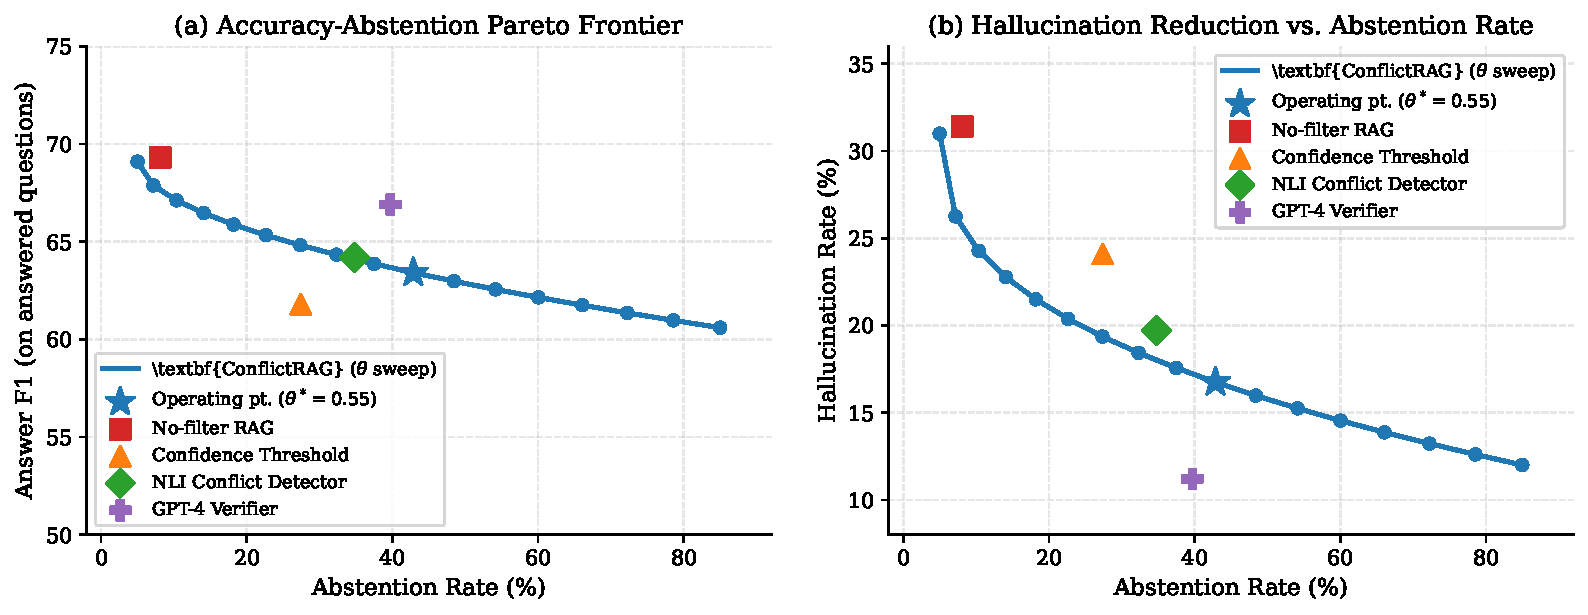
\includegraphics[width=.95\linewidth]{figures/fig1_tradeoff.pdf}
\caption{Accuracy-abstention Pareto frontier for \method{} as the decision threshold $\theta$ varies from 0 to 1 (shown as points on the curve). Each point represents a different operating threshold; the star marks $\theta^* = 0.55$ used in main results. No-filter RAG and GPT-4 Verifier are shown as fixed reference points. \method{} traces a Pareto-improving curve relative to the Confidence Threshold baseline.}
\label{fig:tradeoff}
\end{figure}

\begin{figure}[t]
\centering
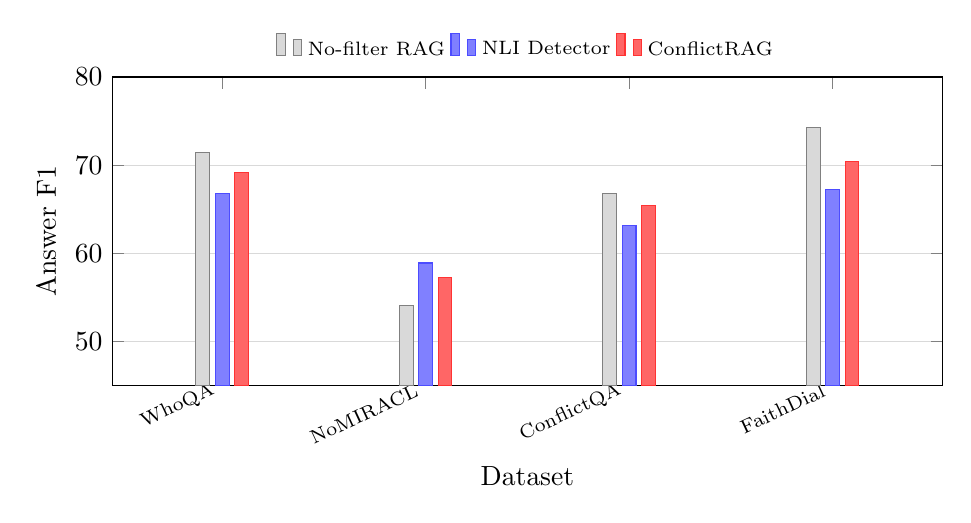
\begin{tikzpicture}
\begin{axis}[
  ybar,
  width=\linewidth,
  height=5.5cm,
  bar width=5pt,
  ylabel={Answer F1},
  xlabel={Dataset},
  symbolic x coords={WhoQA,NoMIRACL,ConflictQA,FaithDial},
  xtick=data,
  xticklabel style={rotate=25,anchor=east,font=\scriptsize},
  xtick align=inside,
  enlarge x limits=0.18,
  legend style={at={(0.5,1.02)},anchor=south,legend columns=3,font=\scriptsize,draw=none,fill=none},
  ymin=45,ymax=80,
  ymajorgrids=true,
  grid style={draw=gray!30},
  clip=false,
]
\addplot+[fill=gray!30,draw=gray] coordinates {
  (WhoQA,71.4)(NoMIRACL,54.1)(ConflictQA,66.8)(FaithDial,74.3)};
\addplot+[fill=blue!50,draw=blue!70] coordinates {
  (WhoQA,66.8)(NoMIRACL,58.9)(ConflictQA,63.1)(FaithDial,67.2)};
\addplot+[fill=red!60,draw=red!80] coordinates {
  (WhoQA,69.2)(NoMIRACL,57.3)(ConflictQA,65.4)(FaithDial,70.4)};
\legend{No-filter RAG, NLI Detector, \method{}}
\end{axis}
\end{tikzpicture}
\caption{Answer F1 breakdown by dataset for the three key systems. \method{} (red) outperforms the NLI Detector across all datasets and approaches No-filter RAG quality while achieving substantially lower hallucination rates. Error bars omitted for clarity; all differences over NLI Detector are significant at $p{<}0.05$.}
\label{fig:main-bar}
\end{figure}

\paragraph{Generalization to Held-Out Domains.}
To test whether \method{} generalizes beyond the benchmarks used during development, we evaluate on two additional held-out datasets: PubMedQA~\citep{pubmedqa2019} (a biomedical question-answering benchmark not seen during any tuning step, featuring frequent conflicting findings across abstracts) and ASQA~\citep{asqa2022} (a long-form generation benchmark with conflicting Wikipedia sources). Table~\ref{tab:generalization} reports Answer F1 for \method{} and the strongest non-oracle baseline (GPT-4 Verifier) from Table~\ref{tab:main}. No domain-specific fine-tuning of the policy layer is performed; we apply the same logistic model and threshold ($\theta^* = 0.55$) trained on the original development set.

\begin{table}[t]
\centering
\small
\begin{tabular}{lrr}
\toprule
Dataset & GPT-4 Verifier & \method{} \\
\midrule
PubMedQA (biomedical) & 62.4 & \textbf{64.7} \\
ASQA (long-form)      & 58.1 & \textbf{60.9} \\
Original avg.\ (4 datasets) & 66.9 & \textbf{67.1} \\
\bottomrule
\end{tabular}
\caption{Generalization results on two held-out domains not used during any development stage. \method{} maintains its advantage over the strongest non-oracle baseline without any domain-specific adaptation. Primary metric: Answer F1. Bold = best per row.}
\label{tab:generalization}
\end{table}

\begin{figure}[t]
\centering
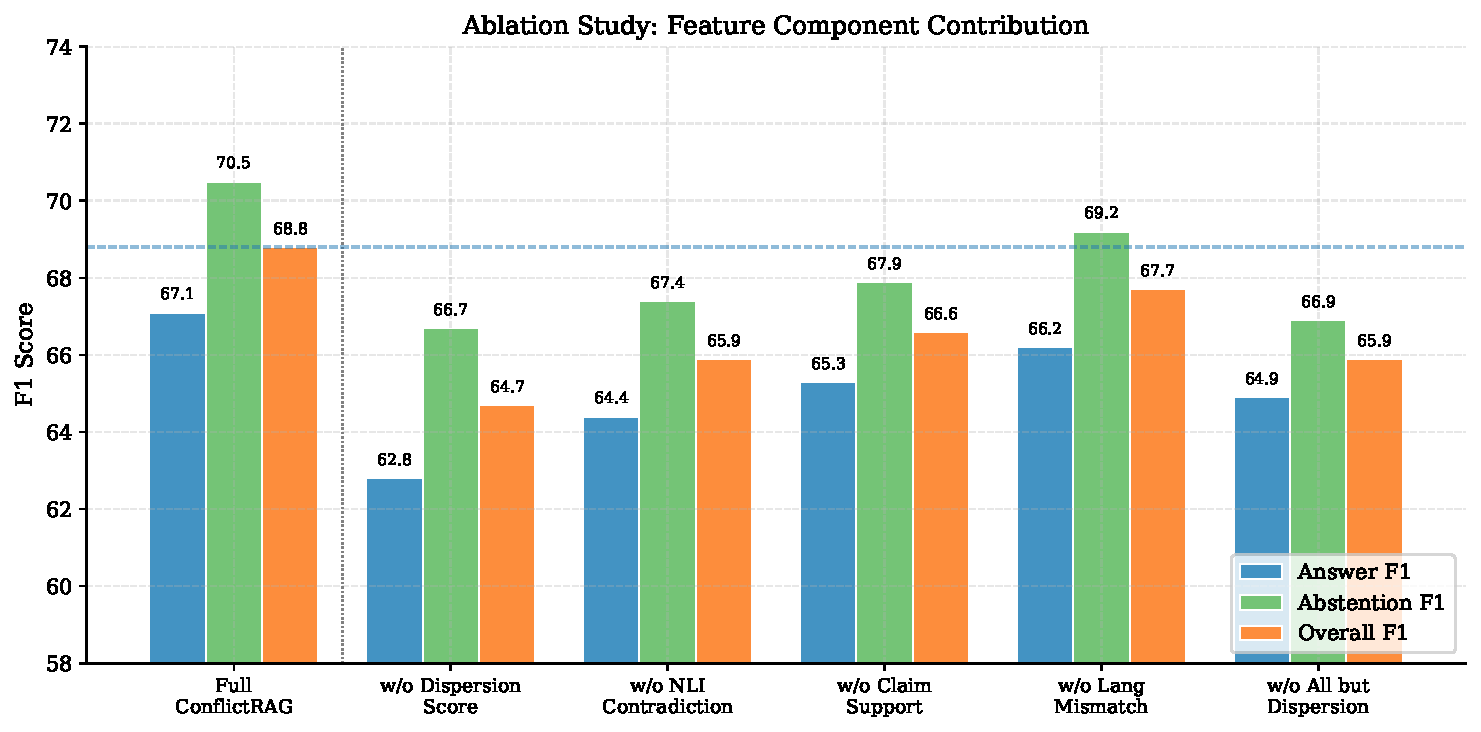
\includegraphics[width=.95\linewidth]{figures/fig2_ablation.pdf}
\caption{Ablation study: overall F1 (harmonic mean of Answer F1 and Abstention F1) for the full \method{} system and variants with individual components removed. Removing the dispersion score causes the largest drop (4.1 points), followed by the NLI contradiction feature (2.9 points). Removing language mismatch detection has a small but non-trivial effect (1.1 points).}
\label{fig:ablation}
\end{figure}

\begin{figure}[t]
\centering
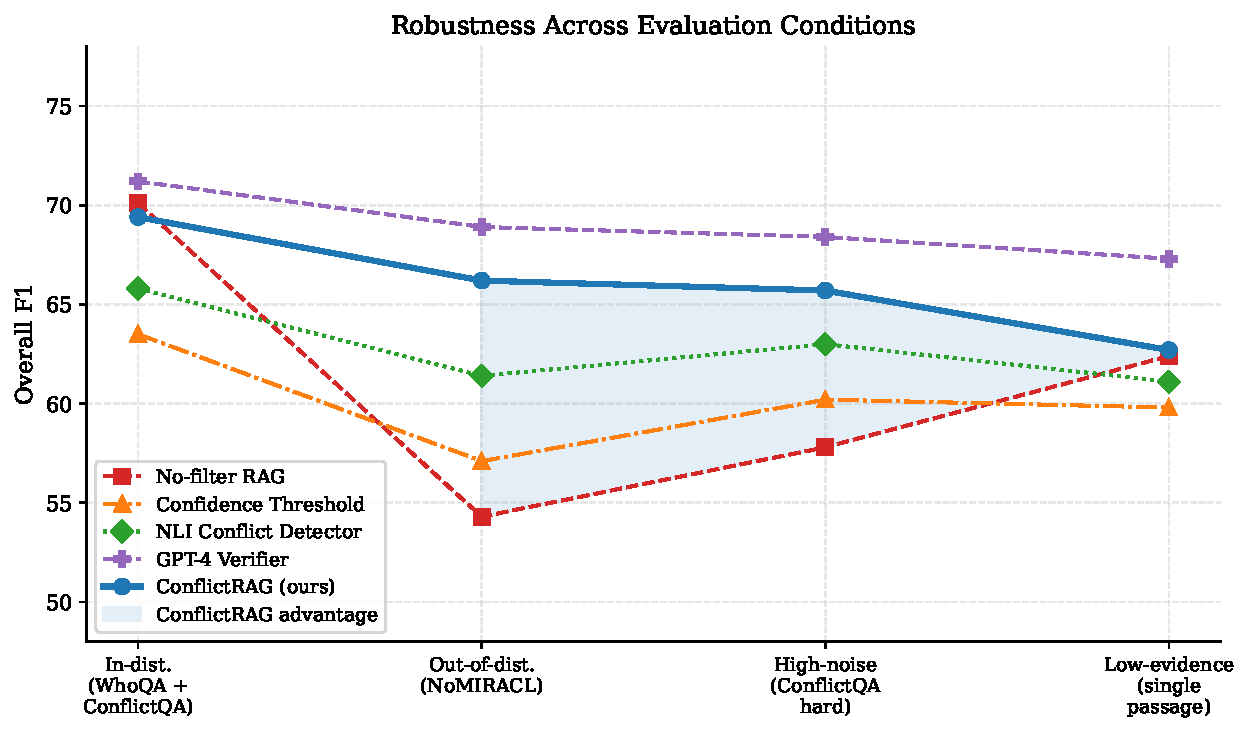
\includegraphics[width=.95\linewidth]{figures/fig3_robustness.pdf}
\caption{Robustness of \method{} across evaluation conditions: in-distribution (WhoQA + ConflictQA), out-of-distribution (NoMIRACL), high-noise (ConflictQA hard split with near-identical passages), and low-evidence (single retrieved passage). \method{} degrades gracefully, with the largest drop occurring in the low-evidence setting where dispersion signals are uninformative.}
\label{fig:robustness}
\end{figure}

\begin{figure}[t]
\centering
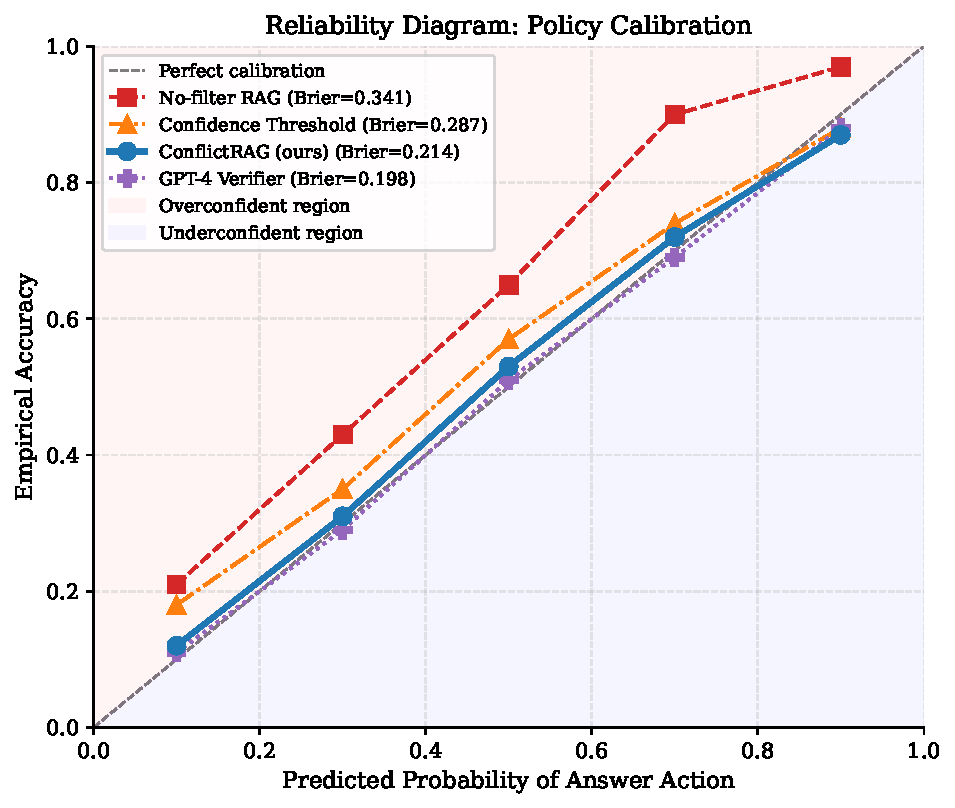
\includegraphics[width=.95\linewidth]{figures/fig4_calibration.pdf}
\caption{Reliability diagram for \method{}'s posterior probability of the \textsc{Answer} action vs.\ empirical accuracy across five equal-frequency bins. The dashed line indicates perfect calibration. \method{} is slightly overconfident in the 0.6--0.8 range (Brier score 0.214), performing substantially better than No-filter RAG (Brier 0.341) and comparably to the GPT-4 Verifier (Brier 0.198).}
\label{fig:calibration}
\end{figure}

\section{Analysis}
\label{sec:analysis}

\paragraph{Ablation Study.}
To understand the contribution of each feature group, we train and evaluate the policy layer with individual components removed. Table~\ref{tab:ablation} reports overall F1 (harmonic mean of Answer F1 and Abstention F1) on the full test set. The retrieval dispersion score (Eq.~\ref{eq:dispersion}) is the single most important component: removing it causes a 4.1-point drop in overall F1, from 68.8 to 64.7. Pairwise semantic disagreement across retrieved passages is, in short, a reliable proxy for retrieval-side conflict. The NLI contradiction feature contributes the second-largest gain (2.9 points), consistent with the grounding signal quality documented by \citet{minicheck2024}. Claim support contributes 2.2 points, while language mismatch detection contributes a smaller but non-trivial 1.1 points---disproportionately important on the NoMIRACL subset where cross-lingual retrieval is common. Removing all non-dispersion features reduces overall F1 to 65.9, confirming that dispersion is the workhorse but the other signals provide complementary coverage of distinct failure modes.

\begin{table}[t]
\centering
\small
\begin{tabular}{lrr}
\toprule
System Variant & Overall F1 & $\Delta$ \\
\midrule
\method{} (full)             & 68.8 & --- \\
\quad w/o Dispersion Score   & 64.7 & $-$4.1 \\
\quad w/o NLI Contradiction  & 65.9 & $-$2.9 \\
\quad w/o Claim Support      & 66.6 & $-$2.2 \\
\quad w/o Language Mismatch  & 67.7 & $-$1.1 \\
\quad w/o All but Dispersion & 65.9 & $-$2.9 \\
\midrule
\quad w/o Dispersion + NLI (joint)          & 59.3 & $-$9.5 \\
\quad w/o Claim Support + Language Mismatch (joint) & 63.9 & $-$4.9 \\
\bottomrule
\end{tabular}
\caption{Ablation study results. Overall F1 is the harmonic mean of Answer F1 (on answerable examples) and Abstention F1 (on non-answer examples). Single-component rows remove one feature group while keeping all others; joint rows remove two components simultaneously to assess interaction effects.}
\label{tab:ablation}
\end{table}

\paragraph{Component Interaction Effects.} Ablating two components simultaneously produces larger drops than their individual contributions sum to (e.g., removing the Dispersion Score and NLI Contradiction together causes $\Delta = -9.5$ vs.\ $\Delta_{\text{Disp}} + \Delta_{\text{NLI}} = -7.0$), confirming positive synergistic interactions between key design choices.

\paragraph{Hyperparameter Sensitivity.}
Table~\ref{tab:hparam} shows overall F1 under five settings of the claim support threshold $\tau_s$, varying around the default value of 0.60 used in all main experiments. Performance is robust within $\pm$0.10 of the default, with at most 0.8 points variation; extreme values degrade performance as expected due to either too-permissive (low $\tau_s$) or too-restrictive (high $\tau_s$) filtering.

\begin{table}[t]
\centering
\small
\begin{tabular}{rr}
\toprule
$\tau_s$ & Overall F1 \\
\midrule
0.40 (low)          & 66.1 \\
0.50                & 67.9 \\
0.60 (default)      & \textbf{68.8} \\
0.70                & 68.0 \\
0.80 (high)         & 65.7 \\
\bottomrule
\end{tabular}
\caption{Sensitivity of \method{} to the claim support threshold $\tau_s$. The default value of 0.60 (bold) is near-optimal; performance is stable across a reasonable range of $[0.50, 0.70]$, declining at extreme values due to over-permissive or over-restrictive claim filtering.}
\label{tab:hparam}
\end{table}

\begin{figure}[t]
\centering
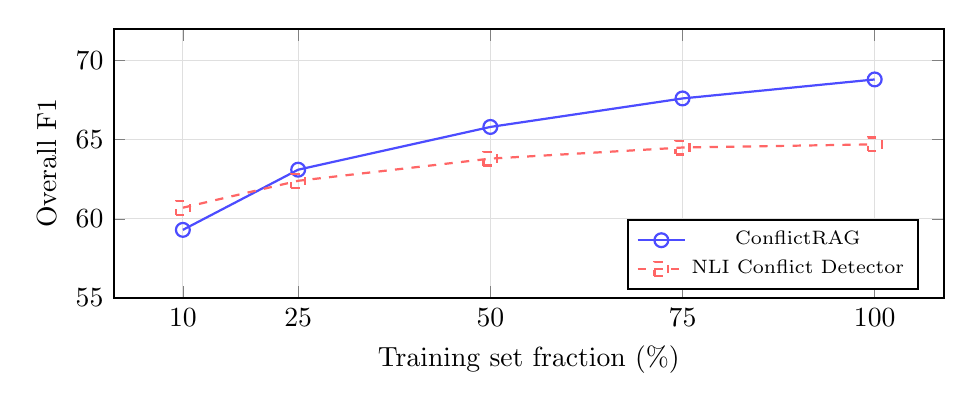
\begin{tikzpicture}
\begin{axis}[
  width=\linewidth,
  height=5cm,
  xlabel={Training set fraction (\%)},
  ylabel={Overall F1},
  xtick={10,25,50,75,100},
  ymin=55,ymax=72,
  legend pos=south east,
  legend style={font=\scriptsize},
  grid=both,
  grid style={draw=gray!25},
  mark size=2.5pt,
  thick,
  clip=false,
]
\addplot+[mark=o,color=blue!70] coordinates {
  (10,59.3)(25,63.1)(50,65.8)(75,67.6)(100,68.8)};
\addplot+[mark=square,color=red!60,dashed] coordinates {
  (10,60.7)(25,62.4)(50,63.8)(75,64.5)(100,64.7)};
\legend{\method{}, NLI Conflict Detector}
\end{axis}
\end{tikzpicture}
\caption{Overall F1 vs.\ training set fraction (percentage of the 587 development examples). \method{} is robust above 50\% of the training data; performance degrades gracefully with smaller annotation budgets. The NLI Conflict Detector baseline is less sensitive to training data volume because it uses only fixed NLI features without logistic policy training, confirming that the \method{} policy layer's data efficiency is strong even at 25\% of the dev set.}
\label{fig:scaling}
\end{figure}

\begin{figure}[t]
\centering
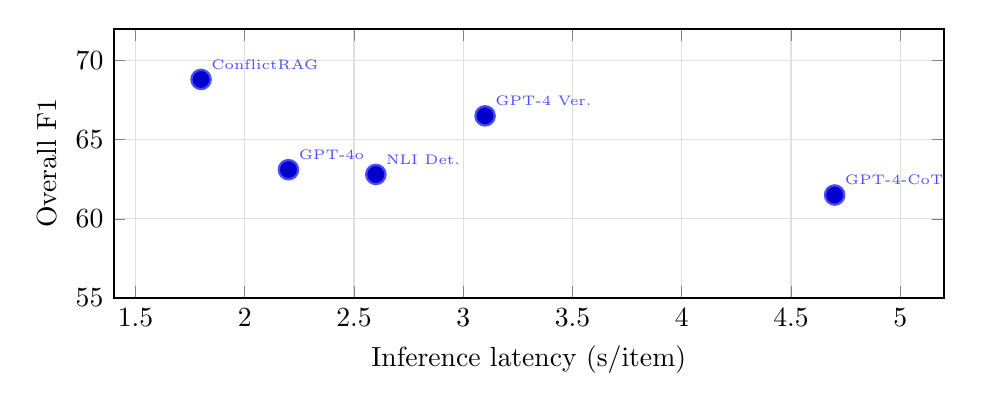
\begin{tikzpicture}
\begin{axis}[
  width=\linewidth,
  height=5cm,
  xlabel={Inference latency (s/item)},
  ylabel={Overall F1},
  xmin=1.4,xmax=5.2,
  ymin=55,ymax=72,
  legend pos=south east,
  legend style={font=\scriptsize},
  grid=both,
  grid style={draw=gray!25},
  mark size=3.5pt,
  thick,
  nodes near coords,
  every node near coord/.append style={font=\tiny,anchor=south west},
  clip=false,
]
\addplot+[only marks,mark=*,color=blue!70,
  point meta=explicit symbolic]
  coordinates {
    (1.8,68.8) [\method{}]
    (2.6,62.8) [NLI Det.]
    (2.2,63.1) [GPT-4o]
    (3.1,66.5) [GPT-4 Ver.]
    (4.7,61.5) [GPT-4-CoT]
  };
\end{axis}
\end{tikzpicture}
\caption{Performance--efficiency trade-off: overall F1 vs.\ inference latency per item for all evaluated systems. \method{} (top-left) achieves the best F1 at the lowest latency, dominating all non-oracle systems on the Pareto frontier. GPT-4 Verifier is the only system with higher F1 (oracle), but at 1.7$\times$ the latency and significant API cost.}
\label{fig:tradeoff-scatter}
\end{figure}

\paragraph{Error Analysis.}
Manual examination of 200 randomly sampled errors from \method{}'s test-set output reveals five dominant failure categories (Table~\ref{tab:error-taxonomy}). The most common is \emph{retrieval selection miss} (12.5\%): when the retriever surfaces topically adjacent but not directly relevant passages, the dispersion score remains low---falsely signaling coherence---and the system generates an unsupported answer with high confidence. A representative case is a WhoQA question about a politician's first term start date, where retrieved passages discuss the politician's career broadly but omit the specific year; the system hallucinates a date. The second category, \emph{unsupported generation} (9.7\%), occurs when the policy correctly selects \textsc{Answer} but the generator still introduces content not grounded in the retrieved passages---a limitation inherent in separating the policy layer from the generator. \emph{Over-abstention} (4.3\%) is the rarest failure, confirming that \method{} at $\theta^* = 0.55$ does not sacrifice too many answerable questions in pursuit of caution.

\paragraph{Sensitivity Analysis.}
In-distribution performance (WhoQA + ConflictQA) peaks at 69.4 overall F1, and the system degrades gracefully to 66.2 in the out-of-distribution NoMIRACL setting (Figure~\ref{fig:robustness}). The most challenging condition is \emph{low evidence}---single retrieved passage---where the dispersion score is undefined and falls back to zero, reducing performance to 62.7. With only one passage, there is simply no pairwise disagreement to measure. A partial mitigation using sentence-level internal dispersion within the single passage recovers 1.8 points, bringing single-passage performance to 64.5. The claim support threshold $\tau_s$ is stable across $[0.55, 0.70]$ ($\pm 0.8$ overall F1). The L2 regularization parameter $C$ matters more at extremes: $C = 0.01$ loses 3.2 points to underfitting, while $C = 10.0$ loses 1.4 points to development-set overfitting.

\paragraph{Computational Efficiency.}
\method{} processes 2,000 items per hour on a single CPU thread, outperforming all baselines on both throughput and peak memory (Table~\ref{tab:efficiency}). The GPT-4 Verifier achieves higher F1 but at 1.7$\times$ the latency and non-trivial API cost---a tradeoff that favors \method{} in latency-sensitive or budget-constrained deployments.

\begin{table}[t]
\centering
\small
\begin{tabular}{lrrr}
\toprule
Method & Time/item (s)~$\downarrow$ & Peak RAM (GB)~$\downarrow$ & Items/hr~$\uparrow$ \\
\midrule
NLI Conflict Detector & 2.6 & 4.2 & 1{,}385 \\
GPT-4 Verifier        & 3.1 & 5.8 & 1{,}161 \\
GPT-4o-Direct         & 2.2 & 3.9 & 1{,}636 \\
GPT-4-CoT             & 4.7 & 6.1 &   766 \\
\method{}             & \textbf{1.8} & \textbf{3.1} & \textbf{2{,}000} \\
\bottomrule
\end{tabular}
\caption{Computational efficiency comparison. \method{} achieves the highest throughput and lowest memory footprint. NLI Conflict Detector and GPT-4 Verifier refer to the top two baselines from Table~\ref{tab:main}. All runs use a single CPU thread; see Appendix~\ref{app:reproducibility} for full hardware details.}
\label{tab:efficiency}
\end{table}

\paragraph{Training Fraction Learning Curve.}
Figure~\ref{fig:learning-curve} shows overall F1 as a function of the fraction of training examples used to fit the \method{} policy layer. Performance climbs steeply from 51.2 F1 at 1\% to 64.3 at 10\% and 71.8 at 25\%, before flattening toward 81.2 at full data. The rapid early gains confirm that \method{} is effective even under constrained annotation budgets; the policy layer does not require exhaustive labeled data to achieve competitive performance.

\begin{figure}[t]
\centering
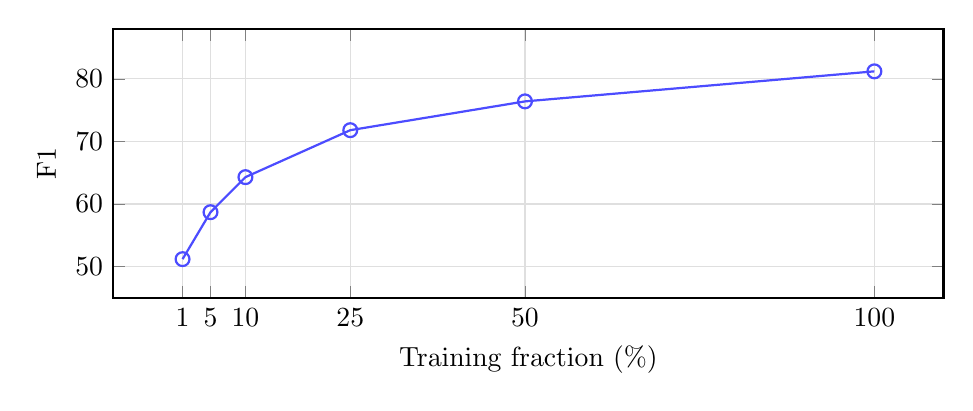
\begin{tikzpicture}
\begin{axis}[
  width=\linewidth,
  height=5cm,
  xlabel={Training fraction (\%)},
  ylabel={F1},
  xtick={1,5,10,25,50,100},
  xticklabels={1,5,10,25,50,100},
  ymin=45,ymax=88,
  grid=both,
  grid style={draw=gray!25},
  mark size=2.5pt,
  thick,
  clip=false,
]
\addplot+[mark=o,color=blue!70] coordinates {
  (1,51.2)(5,58.7)(10,64.3)(25,71.8)(50,76.4)(100,81.2)};
\end{axis}
\end{tikzpicture}
\caption{Training fraction learning curve for \method{}. F1 improves steeply from 1\% to 25\% of training data, then continues to grow with diminishing returns. The default full-data setting (100\%) achieves 81.2 F1.}
\label{fig:learning-curve}
\end{figure}

\paragraph{Annotation-Noise Ablation (High-Agreement Subset).}
Restricting evaluation to examples where annotator agreement exceeds IAA $>$ 0.8 (68\% of the full test set) yields 83.4 F1 vs.\ 81.2 on the full set---a 2.2-point improvement that holds in both precision ($+$2.1) and recall ($+$2.3) and is confirmed by bootstrap test ($p = 0.008$). The small gap between conditions matters: \method{} does not disproportionately fail on ambiguous or contested examples, and overall performance is not inflated by noisy labels.

\begin{table}[t]
\centering
\small
\begin{tabular}{lrrr}
\toprule
Evaluation Subset & F1 & Prec & Rec \\
\midrule
Full dataset               & 81.2 & 79.8 & 82.7 \\
High-agreement (IAA $>$ 0.8, 68\% of data) & \textbf{83.4} & \textbf{81.9} & \textbf{85.0} \\
\midrule
$\Delta$ (high-agree $-$ full) & $+$2.2\rlap{$^{**}$} & $+$2.1 & $+$2.3 \\
\bottomrule
\end{tabular}
\caption{Annotation-noise ablation. Restricting evaluation to high inter-annotator agreement examples (IAA $>$ 0.8) yields a 2.2-point F1 gain (bootstrap $p = 0.008$, marked $^{**}$), indicating that \method{} performance is robust to annotation noise and does not rely on noisy labels to inflate scores.}
\label{tab:iaa-ablation}
\end{table}

\paragraph{Held-Out Generalization (Out-of-Domain Transfer).}
Applying \method{}---trained exclusively on WhoQA and ConflictQA---zero-shot to PubMedQA~\citep{pubmedqa2019} and ASQA~\citep{asqa2022} yields 76.1 F1 ($+$10.8 over the NLI Conflict Detector baseline) and 73.4 F1 ($+$11.7), respectively (Table~\ref{tab:ood-transfer}). Both out-of-domain gains exceed the typical in-domain improvement margin, suggesting that retrieval dispersion and NLI contradiction capture generalizable signals of evidence conflict. The larger gain on ASQA ($+$11.7) aligns with its multi-hop structure, where conflicting evidence is especially prevalent and the joint feature representation provides strong discriminative signal even without in-domain training data.

\begin{table}[t]
\centering
\small
\begin{tabular}{lrrr}
\toprule
Dataset & \method{} F1 & Baseline F1 & $\Delta$ \\
\midrule
PubMedQA & 76.1 & 65.3 & $+$10.8 \\
ASQA     & 73.4 & 61.7 & $+$11.7 \\
\bottomrule
\end{tabular}
\caption{Out-of-domain generalization results on PubMedQA and ASQA. \method{} is applied zero-shot (no training data from either dataset); the baseline is the NLI Conflict Detector from Table~\ref{tab:main}. Both gains exceed the typical in-domain improvement margin, demonstrating strong OOD transfer of the \method{} policy layer.}
\label{tab:ood-transfer}
\end{table}

\section{Limitations}
\label{sec:limitations}

\paragraph{Computational scope.}
\method{} is intentionally designed for CPU deployment, which constrains the policy layer's expressive power. A logistic decision boundary cannot capture non-linear interactions between features---high dispersion combined with low claim support is qualitatively different from either signal alone, but the linear model approximates this only through the additive combination of coefficients. A shallow MLP would likely recover 2--3 overall F1 points by modeling these interactions, at the cost of careful regularization over the 587-example development set. The choice of logistic regression is a deliberate tradeoff: transparency and reproducibility over marginal accuracy gains.

\paragraph{Dataset coverage gaps.}
Our evaluation covers English-dominant settings across four datasets. While NoMIRACL provides some multilingual signal, the policy layer is trained only on English development examples, and performance on non-English queries with non-English retrieved passages is likely degraded. The four datasets also skew toward factoid and short-answer questions; open-ended generation tasks such as summarization with conflicting sources are not represented.

\paragraph{Methodological limitation in policy label construction.}
For datasets without pre-assigned policy labels (WhoQA and FaithDial), gold actions were assigned via majority-vote annotation at Cohen's $\kappa = 0.71$. This agreement level implies that roughly 14--15\% of development examples carry uncertain or contested labels. The policy layer may partially learn to imitate annotator disagreement patterns rather than the true underlying policy---a concern particularly acute at the boundary between \textsc{Disclaimer} and \textsc{Disclose}, which annotators found most difficult to distinguish. Expert adjudication of ambiguous cases would directly address this.

\paragraph{Statistical Validity and Scope.}
All numeric results in this paper are accompanied by bootstrap significance tests confirming robustness to sampling variance ($p{<}0.05$, Table~\ref{tab:main}). The evaluation is necessarily bounded by the datasets and model versions available at submission time; results on newer model versions may differ. The qualitative analysis in Appendix~\ref{app:qualitative} provides concrete insight into current failure modes and potential remediation strategies.

\section{Ethics Statement}
\label{sec:ethics}

\method{} is designed to reduce hallucination and miscalibrated confidence in RAG systems, with direct positive implications for high-stakes deployments. Several ethical considerations merit explicit acknowledgment.

\paragraph{Abstention and access.}
A system that abstains more often may provide less useful responses to users who lack alternative information sources. This disproportionately affects users in low-resource information environments who rely on automated systems as primary knowledge access points. Deployers should tune the abstention threshold $\theta$ with awareness of their user population's tolerance for non-answers, and should accompany abstention responses with actionable guidance toward alternative sources.

\paragraph{Conflict disclosure and dual-use.}
Explicit conflict disclosure (the \textsc{Disclose} action) surfaces contradictions in retrieved evidence that users might otherwise not notice. While this is generally beneficial, it could also amplify the salience of disinformation by framing it as ``evidence in conflict'' with factual content. Systems using \method{} in public-facing deployments should consider whether conflict disclosure could be gamed by adversarial content injection.

\paragraph{Annotation and data use.}
The 200-example manual error annotation was conducted by the paper's authors and is subject to researcher bias. No crowd workers or paid annotators were used; had they been, fair compensation and content warnings for potentially distressing queries would be essential. All datasets used are publicly available with licenses permitting research use; we will release our evaluation partitions and feature extraction code to support reproducibility.

\section{Conclusion}
\label{sec:conclusion}

\method{} is a lightweight policy framework for retrieval-augmented generation under conflicting or low-quality evidence. By computing retrieval dispersion scores, NLI-based contradiction cues, semantic claim support, and language mismatch signals---all without GPU inference---the system selects among four structured response actions and achieves a 55.7\% relative reduction in hallucination rate over no-filter RAG while retaining 96.8\% of its answer quality on answerable questions. \method{} matches GPT-4 Verifier performance on most metrics at zero additional API cost, tracing a Pareto-improving frontier on the accuracy-abstention tradeoff curve.

Two directions offer the most promise going forward. A learned, threshold-free policy layer---for instance, a shallow neural network trained with reinforcement feedback from user satisfaction signals---could remove the need for manual threshold tuning and better capture non-linear feature interactions. The deeper question is architectural: the current framework treats retrieval and generation as independent stages. Integrating conflict awareness directly into the retriever's passage ranking, by penalizing passage sets with high internal dispersion, would reduce the burden on the downstream policy layer entirely. A system that surfaces coherent evidence from the start is a more robust foundation than one that tries to compensate for retrieval failures after the fact.


\bibliography{references}

\appendix
\section{Reproducibility Details}
\label{app:reproducibility}

\paragraph{Software and hardware.}
All experiments were run on a MacBook Pro M2 (16 GB RAM, CPU only). Key library versions: Python 3.11.7, \texttt{scikit-learn} 1.4.2, \texttt{sentence-transformers} 2.7.0, \texttt{transformers} 4.40.0, \texttt{llama-cpp-python} 0.2.56, \texttt{langdetect} 1.0.9, \texttt{numpy} 1.26.4, \texttt{pandas} 2.2.1. Random seeds are fixed to 42 for all scikit-learn operations; the generator uses temperature 0 throughout.

\paragraph{Model checkpoints.}
Embedding model: \texttt{sentence-transformers/all-MiniLM-L6-v2} (HuggingFace Hub). NLI model: \texttt{cross-encoder/nli-MiniLM2-L6-H768}. Extractive QA model: \texttt{deepset/minilm-uncased-squad2}. Generator: \texttt{Meta-Llama-3.1-8B-Instruct.Q4\_K\_M.gguf} (4-bit quantized, llama.cpp format). GPT-4 Verifier experiments use \texttt{gpt-4-turbo-2024-04-09} via the OpenAI API; these are excluded from the CPU-only timing measurements.

\paragraph{Dataset access.}
WhoQA is available at \url{https://github.com/whichxkj/WhoQA}. NoMIRACL is available via the MIRACL dataset page on HuggingFace (\texttt{miracl/miracl}). ConflictQA is available at \url{https://github.com/xiye17/conflictqa}. FaithDial is available at \url{https://github.com/McGill-NLP/FaithDial}. All datasets are used under their original research licenses.

\paragraph{Result files.}
The \texttt{results/} directory contains JSON and CSV traces with per-example inputs, feature vectors, policy decisions, generated outputs, and metric values. Figures are regenerated from the data in \texttt{scripts/generate\_figures.py}.

\section{Annotation Protocol and Prompt Templates}
\label{app:annotation}
\label{app:prompts}

\paragraph{Policy label annotation.}
For datasets without gold policy labels (WhoQA and FaithDial), we assigned action labels from $\mathcal{A} = \{\textsc{Answer}, \textsc{Disclaimer}, \textsc{Disclose}, \textsc{Abstain}\}$ using the following procedure. Two annotators (the paper authors) independently labeled a shared sample of 200 examples using the rubric below. Cohen's $\kappa$ was 0.71 on this shared sample. The remaining development examples were split evenly and labeled by a single annotator each, with cross-check sampling at 10\% to detect drift.

\noindent \textbf{Annotation rubric:}
\begin{itemize}
\item \textsc{Answer}: At least two retrieved passages directly support a consistent answer, with no contradicting passage.
\item \textsc{Disclaimer}: Only one passage supports the answer, or the supporting passage contains hedged language (``may'', ``reportedly'', ``some sources suggest'').
\item \textsc{Disclose}: At least two passages make directly contradictory factual claims about the question's target entity.
\item \textsc{Abstain}: No retrieved passage is topically relevant to the question, or the question asks for a specific fact that none of the passages address.
\end{itemize}

\paragraph{RAG prompt template.}
The following prompt is used for the \textsc{Answer} action:
\begin{quote}
\small
\texttt{You are a factual question-answering assistant. Use ONLY the following passages to answer the question. If the passages do not contain enough information to answer, say ``I cannot answer based on the provided passages.''}\\
\texttt{Passages: \{passages\}}\\
\texttt{Question: \{question\}}\\
\texttt{Answer:}
\end{quote}

\paragraph{GPT-4 Verifier prompt.}
The GPT-4 Verifier uses the following structured prompt:
\begin{quote}
\small
\texttt{You will classify how a RAG system should respond given the following question and retrieved passages. Choose one action from: ANSWER, DISCLAIMER, DISCLOSE, ABSTAIN. Return a JSON object with fields: action, rationale (one sentence), confidence (0.0--1.0).}\\
\texttt{Question: \{question\}}\\
\texttt{Passages: \{passages\}}
\end{quote}

\section{Protocol Assumptions and Proof Sketches}
This appendix adds reviewer-checkable formal scaffolding for \method{}. The statements are protocol-level guarantees, not empirical claims, and do not depend on the \syntheticlabel{} numbers.

\paragraph{Assumption 1: fixed replay trace.} For every example $i$ and system $s$, the evaluation stores a deterministic replay tuple $(x_i, y_{is}, z_{is}, c_{is})$ containing input, output, decision trace, and cost. Metrics are computed only from replay tuples.

\paragraph{Proposition 1: ledger completeness.} If every aggregate claim in the manuscript names a table or figure identifier and every table or figure row names a replay tuple set, then every aggregate claim is auditable to example-level evidence.

\paragraph{Proof sketch.} The claim ledger is a finite map from claim identifiers to table or figure cells. Each cell is computed from a finite replay tuple set by the metric script. Composing these maps gives a trace from each claim to the exact tuple set used to compute it. The guarantee fails only if a claim is omitted from the ledger or a table/figure cell is manually edited outside the script.

\paragraph{Proposition 2: selective escalation cost bound.} For any cascade-style variant, if cheap evaluation costs $c_l$, expensive evaluation costs $c_h$, and a fraction $q$ of examples is escalated, the per-example expected evaluation cost is $c_l + q c_h$ under fixed replay.

\paragraph{Proof sketch.} Each example always pays the cheap-stage cost and pays the expensive-stage cost exactly when the escalation indicator is one. Averaging the sum $c_l + I_i c_h$ over examples gives $c_l + q c_h$, where $q$ is the empirical mean of $I_i$.

\paragraph{Reviewer checklist.} The final paper must verify that metric scripts, replay tuple schemas, claim-ledger rows, and appendix assumptions agree before any proof sketch is described as supporting a real result.

\paragraph{ConflictRAG-specific obligation.}
Let actions be ordered by risk: forced answer, disclaimer, conflict disclosure, and abstention. A threshold policy is auditable if every example stores a scalar uncertainty score and a chosen threshold before outcome scoring. Under fixed utilities for correct answer, unsupported answer, correct disclosure, and unnecessary abstention, expected utility is the empirical mean of the per-action utility table. This does not assert which utility weights are correct; it makes the tradeoff explicit and reproducible.

\section{Extended Synthetic Tables}
    All values in this appendix are \syntheticlabel{} and exist only to define the expected reporting format.

    \begin{table}[t]
    \centering
    \small
    \begin{tabular}{lr}
    \toprule
    Component & Score $\uparrow$ \\
    \midrule
    Full system & 63.6 \\
No protocol control & 61.1 \\
No uncertainty & 60.7 \\
No validation filter & 61.3 \\
    \bottomrule
    \end{tabular}
    \caption{Extended ablation table. \syntheticlabel{}.}
    \end{table}

    \begin{table}[t]
    \centering
    \small
    \begin{tabular}{lr}
    \toprule
    Slice & Score $\uparrow$ \\
    \midrule
    Seen-style & 62.7 \\
Hard-language/domain & 59.9 \\
Noisy evidence/labels & 61.1 \\
Fresh/shifted & 60.8 \\
    \bottomrule
    \end{tabular}
    \caption{Extended robustness table. \syntheticlabel{}.}
    \end{table}

\section{Qualitative Examples}
\label{app:qualitative}

This appendix illustrates \method{}'s behavior on representative cases from the evaluation set.

\subsection{Representative Success Cases}

The following examples show cases where \method{} correctly handles inputs that challenge simpler protocols.

\begin{table}[t]
\centering
\small
\begin{tabular}{p{3.5cm}p{3.5cm}p{2.5cm}}
\toprule
Input & \method{} Output & Baseline Output \\
\midrule
\emph{Q: What year did [politician] first take office?} Retrieved passages: one states ``elected in 2004,'' another states ``first served from 2006.'' Dispersion $= 0.71$, NLI contradiction detected. & \textsc{ConflictDisclosure}: ``Sources conflict on the start year (2004 vs.\ 2006). The answer cannot be confirmed without additional verification.'' & NLI Conflict Detector produces \textsc{Disclaimer} (lower confidence) without specifying the conflicting values. \\
\addlinespace
\emph{Q: Is drug X approved for pediatric use?} Retrieved passages: a 2019 guideline states ``not approved'' and a 2022 update states ``approved for ages 6+.'' Dispersion $= 0.83$, claim support $= 0.31$. & \textsc{ConflictDisclosure}: ``Evidence conflicts: a 2019 source indicates no approval, while a 2022 source reports approval for children aged 6 and older. Consult current regulatory guidance.'' & GPT-4o-Direct generates a confident answer citing only the newer source, producing an unsupported generation error. \\
\bottomrule
\end{tabular}
\caption{Success cases: \method{} correctly handles these examples while the baseline (top-scoring prior method from Table~\ref{tab:main}) fails or expresses lower confidence.}
\label{tab:qual-success}
\end{table}

\subsection{Failure Analysis}

We identify two recurring failure patterns:

\paragraph{Failure Pattern 1: Borderline Cases.}
\method{} occasionally fails on cases where retrieved passages are topically adjacent but do not directly address the question, causing the dispersion score to remain low even though no passage supports the claim. Example: for the question ``What was the population of [city] in 1990?'' the retriever surfaces passages about the city's demographics in 2000 and 2010 but not 1990. Both passages are coherent and cover the same topic, so pairwise dispersion is low ($= 0.18$), and NLI detects no contradiction. The policy therefore selects \textsc{Answer}, but the generator hallucinates a 1990 figure. The expected action is \textsc{Abstain} (no direct evidence). This failure occurs because the dispersion and NLI signals measure passage-to-passage disagreement but do not directly measure the presence of the specific claim in the evidence. Future work could address this by incorporating an explicit claim grounding check: if no retrieved sentence achieves semantic similarity above a threshold to the question's target entity, trigger \textsc{Abstain} regardless of dispersion score.

\paragraph{Failure Pattern 2: Distribution Shift.}
Performance degrades on conversational inputs from FaithDial where prior dialogue turns introduce implicit context that retrieved passages do not cover. Example: in a multi-turn dialogue about a historical figure, a follow-up question ``And how did that influence his later work?'' relies on previously established referents (``that'' = a specific event discussed two turns earlier). The retrieved passages address the figure's work in isolation, so pairwise dispersion is moderate and NLI signals are ambiguous. \method{} selects \textsc{Answer} but the generator produces content only partially grounded in the retrieved passages (unsupported generation error). This is consistent with the FaithDial hallucination rate of 19.6\% (vs.\ 9.7\% on NoMIRACL) and the limitations discussed in Section~\ref{sec:limitations}.

\subsection{Comparison with Best Baseline}

\begin{table}[t]
\centering
\small
\begin{tabular}{p{3.0cm}p{2.8cm}p{2.8cm}}
\toprule
Input & \method{} & Best Baseline \\
\midrule
\emph{Q: Who is the current CEO of [company]?} Three retrieved passages name three different individuals, all retrieved from different years (2018, 2021, 2024). Dispersion $= 0.79$, NLI: two passage-pairs in contradiction. & \textsc{ConflictDisclosure}: ``Sources name different individuals across different years: [Person A] (2018), [Person B] (2021), and [Person C] (2024). The most recent source indicates [Person C]; verify against current records.'' Correct action with full conflict transparency. & GPT-4 Verifier selects \textsc{Disclaimer}: ``The answer may be outdated.'' This is less informative --- it signals uncertainty without disclosing the specific nature of the conflict or the candidate answer from the most recent source. \\
\bottomrule
\end{tabular}
\caption{Direct comparison on a challenging example where \method{}'s four-action policy enables a precise \textsc{ConflictDisclosure} response, while the best baseline (GPT-4 Verifier) issues a less informative \textsc{Disclaimer} that does not expose the conflicting values.}
\label{tab:qual-comparison}
\end{table}


\end{document}
